En este episodio vamos a hablar de \emph{resaltado de sintaxis}, es
decir, vamos a aprender a darle formato al código fuente que hayamos
insertado en nuestro documento con la idea de que sea más fácil de leer.

Hay varios paquetes que nos permiten pintar de colorines nuestro código,
está
\href{http://www.ctan.org/tex-archive/macros/latex/contrib/listings/}{\lstinline!listings!}
que he usado bastante,
\href{http://www.ctan.org/tex-archive/macros/latex/contrib/minted/}{\lstinline!minted!}
que tenía ganas de aprender a usar y
\href{http://www.ctan.org/pkg/lgrind}{\lstinline!LGrind!} que descubrí
al escribir esto. Voy a hablar de los dos primeros que son los que
controlo y sobre \lstinline!LGrind! investigáis si os gusta, igual hasta
hay más por ahí.

\section{Lo fácil: listings}

El paquete \lstinline!listings! se utiliza de manera similar al resto de
paquetes que hemos visto hasta ahora: lo cargamos, establecemos sus
opciones y luego utilizamos los comandos que nos proporciona en el
cuerpo del documento.

Para incluir el código hay varias opciones. Por una parte, igual que
ocurría con las ecuaciones y las figuras, podemos escribir código en la
propia línea (\emph{inline}) o puede flotar. Y también como en el caso
de las figuras y ecuaciones, al código flotante podemos ponerle un
\emph{pie de código} (\lstinline!caption!) y etiquetarlo
(\lstinline!label!) para luego referenciarlo en el texto
(\lstinline!\ref{}!).

Para incluir código \emph{inline} tenemos el comando
\lstinline!\lstinline!, muy útil él para hacer referencia a órdenes y
variables en el texto:

\begin{lstlisting}[language={[latex]tex}]
Guardamos el resultado en la variable \lstinline!fib!
\end{lstlisting}

Los signos de exclamación delimitan el código y pueden sustituirse por
cualquier otro carácter no incluido en el código.

Para escribir código con línea propia está el entorno
\lstinline!lstlisting!, al que le podemos dar como opciones tanto el
\emph{pie de código} y su posición como la etiqueta del pedacito de
código:

\begin{lstlisting}[language={[latex]tex}]
% Código con pie en la parte inferior (por defecto en la superior) y etiqueta
\begin{lstlisting}[language=haskell, caption=Código con Listings, captionpos=b, label=lst:fiboHaskell]
  -- Fibonacci!
  fib = 0 : 1 : zipWith (+) fib (tail fib)
\_end{lstlisting}
\end{lstlisting}

Por otra parte, se puede escribir el código en el propio documento o
importarlo de un archivo externo.

\begin{lstlisting}[language={[latex]tex}]
\lstinputlisting[language={[latex]tex}]{Codigo/codigo.tex}
\end{lstlisting}

He puesto precisamente un ejemplo de LaTeX porque tiene una
característica especial: es un \emph{dialecto} de TeX, así veis cuál es
la sintaxis para indicar dialectos.

Este comando es especialmente interesante con los argumentos opcionales
\lstinline!firstline! y \lstinline!lastline! mediante los cuales le
indicamos a LaTeX el trozo de programa que nos interesa pintar:

\begin{lstlisting}[language={[latex]tex}]
\lstinputlisting[language={[latex]tex}, firstline=5, lastline=10]{Codigo/codigo.tex}
\end{lstlisting}

Al igual que con el entorno \lstinline!lstlisting!, al código importado
mediante \lstinline!\lstinputlsiting! podemos ponerle un \emph{pie de
código} con el argumento opcional \lstinline!caption!. Por cierto, si
queremos, podemos recopilar todos los listados de código flotantes en un
índice con el comando \lstinline!\lstlistoflistings!, del mismo modo que
hacíamos con las tablas y las figuras.

Pasemos ahora a personalizarlo. Si no especificamos nada,
\lstinline!listings! nos pintará los comentarios en cursiva, las
palabras claves en negrita y demás, pero todo ello en blanco y negro. Si
queremos otro tipo de formato o usar diferentes colores necesitamos
indicárselo. Veamos cómo se hace.

Lo primero es cargar el paquete \lstinline!xcolor! que, como sabemos de
entregas anteriores nos permite usar colores en nuestro documento:

\begin{lstlisting}[language={[latex]tex}]
\usepackage[usenames,dvipsnames,svgnames,table]{xcolor}
\end{lstlisting}

Luego, en el cuerpo del documento definimos el estilo de nuestro código
con \lstinline!\lstset{OPCIONES}!. Os pongo un ejemplo con diferentes
opciones pero hay muchísimas, lo mejor es mirar en el
\href{http://osl.ugr.es/CTAN/macros/latex/contrib/listings/listings.pdf}{manual}:

\begin{lstlisting}[language={[latex]tex}]
\lstset{
    tabsize=2, % tab = 2 espacios
    backgroundcolor=\color[HTML]{F0F0F0}, % color de fondo
    captionpos=b, % posición de pie de código, b=debajo
    basicstyle=\ttfamily, % estilo de letra general
    columns=fixed, % columnas alineadas
    extendedchars=true, % ASCII extendido
    breaklines=true, % partir líneas
    prebreak = \raisebox{0ex}[0ex][0ex]{\ensuremath{\hookleftarrow}}, % marcar final de línea con flecha
    showtabs=false, % no marcar tabulación
    showspaces=false, % no marcar espacios
    keywordstyle=\bfseries\color[HTML]{007020}, % estilo de palabras clave
    commentstyle=\itshape\color[HTML]{60A0B0}, % estilo de comentarios
    stringstyle=\color[HTML]{4070A0}, % estilo de strings
}
\end{lstlisting}

¿Recordáis que hablamos en su momento de las diferentes familias, series
y formas de las letras? ¿Y de que había dos maneras para aplicarlas?
Aquí se ve clara la utilidad, usamos \lstinline!\bfseries! en lugar de
\lstinline!\textbf! porque \emph{ya estamos dentro de un grupo}.

También tenemos la opción de definir diferentes estilos mediante el
comando \lstinline!\lstdefinestyle{NOMBRE}{ESTILO}! para luego
aplicarlos con la opción \lstinline!style!. A mí en concreto esta
característica me resultó muy útil en la tesis para poder resaltar mejor
el código de Python específico que se usa en Abaqus (¡programa no libre!
¡Huid!), de esta manera tenía un estilo general que se aplicaba a todos
los listados de código y luego unas pocas opciones más que solo se
aplicaban cuando eran necesarias:

\begin{lstlisting}[language={[latex]tex}]
\lstdefinestyle{abaqusPython}{
    language=python,
    % Palabras clave extra
    morekeywords={CONTINUOUS,NUMBER,MESH,par,name,ParStudy,
    template,define,sample,combine, generate},
    % Delimitadores extra, s porque hay uno a cada lado
    moredelim=[s][\ttfamily\color{magenta}]{<}{>},
}

\lstinputlisting[style=abaqusPython]{calculo.py}
\end{lstlisting}

Por último, tenemos que tener en cuenta que \lstinline!listings! no
acepta UTF8 por lo que no nos va a escribir los caracteres acentuados
directamente. Para solucionar esto lo más sencillo es crear un
\lstinline!\lstset! con la opción \lstinline!literate!, que sirve para
sustituir elementos en el código. En sí, \lstinline!literate! se usa
para que el código pueda
\href{https://en.wikipedia.org/wiki/Literate_programming}{leerse con
mayor facilidad}, pero a nosotros nos viene bien para cada vez que vea
\lstinline!á! lo sustituya por \lstinline!\'a! y nos queden bien los
acentos. Os copio aquí lo que yo uso, tenéis una versión con más
chirimbolos
\href{https://en.wikibooks.org/wiki/LaTeX/Source_Code_Listings\#Encoding_issue}{aquí}:

\begin{lstlisting}[language={[latex]tex}]
% Listings no acepta UTF8
{original}{sustitución}{tamaño}
\lstset{literate=
  {á}{{\'a}}1
  {é}{{\'e}}1
  {í}{{\'i}}1
  {ó}{{\'o}}1
  {ú}{{\'u}}1
  {Á}{{\'A}}1
  {É}{{\'E}}1
  {Í}{{\'I}}1
  {Ó}{{\'O}}1
  {Ú}{{\'U}}1
  {ñ}{{\~n}}1
  {ü}{{\"u}}1
  {Ü}{{\"U}}1
}
\end{lstlisting}

La principal debilidad que se le achaca al paquete \lstinline!listings!
es la de no ser un \emph{lexer} completo, es decir, que no distingue
todos los elementos del lenguaje. Para solucionar este problema tenemos
el paquete \lstinline!minted!.

\section{Lo no tan fácil: minted}

El paquete \lstinline!minted! utiliza
\href{http://pygments.org/}{Pygments}, un resaltador de sintaxis general
escrito en Python, para dar formato al código. Está basado además en el
paquete \href{http://www.ctan.org/pkg/fancyvrb}{\lstinline!fancyvrb!}
(\emph{Fancy Verbatim}), un paquete para dar formato al texto
\emph{verbatim}, osease, al \emph{texto tal cual, sin interpretar las
marcas}.

Digo que no es tan fácil porque requiere una etapa de compilación
intermedia y requiere tener Python 2.6 o superior y Pygments instalados.
Para saber si tenemos Pygments instalado podemos buscar el ejecutable
con \lstinline!whereis pygmentize!, que es la
\href{http://pygments.org/docs/cmdline/}{herramienta para el terminal}
de Pygments. Si no lo tenemos siempre nos queda
\lstinline!pip install pygments!.

Que sea un poco más lío de instalar y usar nos da unas ventajas nada
desdeñables:

\begin{itemize}
\item
  Hay disponibles un mayor número de
  \href{http://pygments.org/languages/}{lenguajes}. ¡Hay hasta
  resaltador de
  \href{https://es.wikipedia.org/wiki/Brainfuck}{BrainFuck}!
\item
  Es más fácil de personalizar
\item
  Acepta UTF8, al menos con \lstinline!xelatex! y
  \lstinline!polyglossia!, y hay posibilidad de elegir la codificación a
  partir de su versión 2.0
\item
  Está bien mantenido, hay mejoras del 2016.
\end{itemize}

Evidentemente, también tiene sus desventajas:

\begin{itemize}
\item
  Hay que compilar con la opción
  \href{https://tex.stackexchange.com/questions/20444/what-are-immediate-write18-and-how-does-one-use-them}{\lstinline!-shell-escape!}
  para que LaTeX permita la ejecución de un programa externo, lo que
  implica ciertos \href{https://0day.work/hacking-with-latex/}{problemas
  de seguridad}.
\item
  La versión\footnote{Podemos ver la versión del paquete que estamos
    usando en el archivo \emph{.log}} de los repositorios suele ser
  antigua, con lo que nos perdemos las últimas funcionalidades como la
  de elegir la codificación. Además, es un poco de lío actualizarlo
  porque requiere
  \href{https://www.ctan.org/pkg/fvextra}{\lstinline!fvextra!} y en
  algunos repos no está.
\end{itemize}

Vayamos a su uso. La opción más básica es usar el entorno
\lstinline!minted! junto con el lenguaje del código en cuestión:

\begin{lstlisting}[language={[latex]tex}]
\begin{minted}{python}
 for n in range(10):
   if n%2:
     print n
\end{minted}
\end{lstlisting}

Que tiene la versión reducida \lstinline!\mint! si el código que
queremos añadir tiene solo una línea. Para delimitar el código podemos
usar diferentes caracteres, los elegimos según los delimitadores que use
nuestro código.

\begin{lstlisting}[language={[latex]tex}]
\mint{python}|print [n for n in range(10) if n%2]|
\end{lstlisting}

Tanto para el caso del entorno \lstinline!minted! como para el comando
\lstinline!\mint! el código tendrá línea propia, pero no se le puede
considerar flotante, para ello debemos rodear cualquiera de las dos
opciones con el entorno \lstinline!listing!, más abajo hay un ejemplo
completo en el que se muestra cómo hacerlo.

Este paquete también nos permite incluir código \emph{inline}:

\begin{lstlisting}[language={[latex]tex}]
Guardamos el resultado en la variable \mintinline{python}{fib}
\end{lstlisting}

Y también tenemos la opción de importar el código tal y como hacíamos
con \lstinline!listings!:

\begin{lstlisting}[language={[latex]tex}]
\inputminted{python}{fibonacci.py}
\end{lstlisting}

Lo más difícil de usar de \lstinline!minted! es llamar al comando que
compilará en documento con la opción \lstinline!-shell-escape!, por
ejemplo:

\begin{lstlisting}[language=bash]
pdflatex -shell-escape documento.tex
\end{lstlisting}

Los que compiláis a pelo o con un Makefile no tenéis problema, los que
estáis usando un editor específico para LaTeX seguramente podréis crear
un comando personalizado para compilar. En Kile, que es el programa que
yo uso ahora mismo, tendríamos que ir a \emph{Settings \textgreater{}
Configure Kile \textgreater{} Tools \textgreater{} Build} y crear una
nueva herramienta de compilación que incluya \lstinline!-shell-escape!
siguiendo el ejemplo del resto de herramientas. Digo una \emph{nueva}
porque no es demasiado recomendable compilar alegremente cualquier
documento con la opción \lstinline!-shell-escape! ya que con TeX se
puede programar \emph{cualquier cosa}, hasta cosas malignas.

Para personalizar el código tenemos diferentes opciones:

\begin{itemize}
\item
  Con \lstinline!\usemintedstyle[LENGUAJE]{ESTILO}! elegimos el
  \href{https://help.farbox.com/pygments.html}{estilo de Pygments} con
  el queremos dar formato al código. Como veis el lenguaje es opcional,
  podemos elegir un estilo para cada lenguaje si nos apetece. Para ver
  los estilos instalados escribimos \lstinline!pygmentize -L styles! en
  el terminal. También podemos definir nuestro propio estilo siguiendo
  las \href{http://pygments.org/docs/styles/}{directrices de Pygments}.
\item
  Los comandos \lstinline!\setminted[LENGUAJE]{ESTILO}! y
  \lstinline!\setmintedinline[LENGUAJE]{ESTILO}!, que tiene precedencia,
  también valen para definir los estilos. El primero afecta al entorno
  \lstinline!minted! y al comando \lstinline!\mint! y el segundo al
  código \emph{inline}.
\item
  El comando \lstinline!\newminted[NOMBRE]{LENGUAJE}{OPCIONES}! nos
  permite guardar las opciones para un determinado lenguaje para el
  entorno \lstinline!minted!. Es similar a \lstinline!\lstdefinestyle!
  del paquete \lstinline!listings!. Si no le ponemos nombre llamará
  \lstinline!LENGcode! a nuestro nuevo estilo donde \lstinline!LENG! es
  el lenguaje del mismo. Para usarlo no tenemos más que sustituir el
  nombre del lenguaje por el del estilo que hemos definido en el entorno
  \lstinline!minted!.
\item
  El comando \lstinline!\newmint[NOMBRE]{LENGUAJE}{OPCIONES}! es el
  equivalente a \lstinline!\newminted! para el comando
  \lstinline!\mint!. Funciona exactamente igual excepto por que
  sustituye \lstinline!\mint! por el nombre que le hemos dado al estilo.
\end{itemize}

\begin{lstlisting}[language={[latex]tex}]
\newmint[py]{python}{bgcolor=black}

\py|print [n for n in range(10) if n%2]|
\end{lstlisting}

En cuanto a las opciones, hay montones de ellas, muchas coinciden con
las de \lstinline!listings!, creo que lo mejor es ir al
\href{http://osl.ugr.es/CTAN/macros/latex/contrib/minted/minted.pdf}{manual}
y mirar, se entiende bastante bien y no es demasiado largo.

¡Veamos un ejemplo completo! Tiene las siguientes características:

\begin{itemize}
\item
  Es un objeto flotante con opción de posición H (\emph{here})
\item
  Crea un índice de codigo con \lstinline!\listoflistings!, el
  equivalente a \lstinline!\lstlistoflistings!
\item
  Activa los números de línea con la opción \lstinline!linenos!
\item
  Nos deja escribir ecuaciones en los comentarios del código gracias a
  \lstinline!mathescape!
\item
  Nos permite escribir en LaTeX dentro de los comentarios del código
  gracias a \lstinline!texcl!. Esta opción se ha convertido en
  \lstinline!texcomments! a partir de la versión 2.0. En este caso lo
  uso para poder enlazar la página web.
\end{itemize}

\begin{lstlisting}[language={[latex]tex}]
% Cambiamos Listing por Listado
\renewcommand{\listingscaption}{Listado}
\listoflistings

\begin{listing}[H]
  \begin{minted}[linenos,mathescape,texcl]{clojure}
  ;; Fibonacci por cortesía de \href{https://pfctelepathy.wordpress.com/}{Ekaitz}
  ;; $F_n = F_{n-1} + F_{n-2} \,/\, F_0 = 0 \wedge F_1 = 1$
  (defn fibo
      ([] (fibo 0 1))
      ([one two]
          (lazy-seq (cons one (fibo two (+ one two))))))
  \end{minted}
  \label{lst:fibo}
  \caption{Código con Minted}
\end{listing}
\end{lstlisting}

Que quedaría así:

\begin{figure}[htbp]
\centering
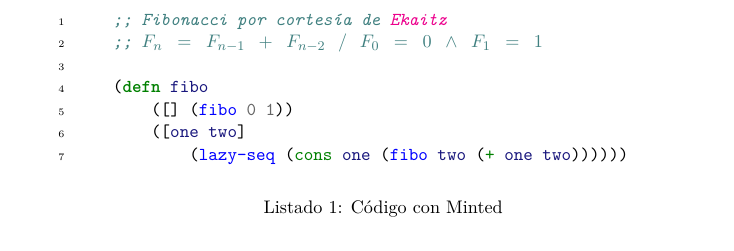
\includegraphics[width=\textwidth]{docs/Figuras/fibo.png}
\caption{Ejemplo de uso de minted}
\end{figure}

Como nota final, \lstinline!listings! no sabe resaltar Clojure y nos
obligaría a crear
\href{http://alexott.net/common/clojure/clj-latex.txt}{nuestro propio
\emph{resaltador}}.

\section{En resumen}\label{en-resumen}

En esta entrega hemos aprendido a resaltar código de dos maneras, una de
ellas usa un paquete de la forma tradicional y la otra llama a un
programa externo. Ambas nos dan una funcionalidad similar siendo tal vez
\lstinline!listings! más fácil de usar y \lstinline!minted! más fácil de
personalizar. Los dos paquetes tienen montones de opciones pero como ya
estamos curtidos, !podemos ir a sus respectivos manuales y leerlos para
saber sacar el máximo partido!

\section{Referencias}\label{referencias}

\href{http://www.texdoc.net/texmf-dist/doc/latex/listings/listings.pdf}{Manual
de \lstinline!listings!}

\href{https://github.com/gpoore/minted}{\lstinline!minted! en GitHub}

\href{http://osl.ugr.es/CTAN/macros/latex/contrib/minted/minted.pdf}{Manual
de \lstinline!minted!}

\href{http://www.tex.ac.uk/FAQ-codelist.html}{\emph{Code listings in
LaTeX} en el FAQ de LaTeX}

\href{https://www.sharelatex.com/learn/Code_listing}{\emph{Code listing}
en ShareLaTeX}

\href{https://tex.stackexchange.com/questions/102596/minted-vs-texments-vs-verbments\#103471}{\lstinline!minted!
vs \lstinline!textments! vs \lstinline!verbments! en TeXExchange}

\href{https://www2.cs.uic.edu/~s/papers/tex2010/}{\emph{Are Text-Only
Data Formats Safe? Or, Use This LaTeX Class File to Pwn Your Computer}}
